\documentclass{article}
\usepackage{cmap}
\usepackage[utf8]{inputenc}
\usepackage[english,ukrainian]{babel}
\usepackage{graphicx}
\usepackage{geometry}
\usepackage{listings}
\usepackage{amsmath}
\usepackage{float}
\geometry{
	a4paper,
	left=20mm,
	right=20mm,
	top=20mm,
	bottom=20mm
}
\lstset{
	language=c,
	tabsize=4,
	keepspaces,
	showstringspaces=false,
}
\graphicspath{ {./pictures} }
\setlength{\parindent}{4em}

\newcommand\subject{Операційні системи}
\newcommand\lecturer{старший викладач кафедри ПЗ\\Грицай О.Д.}
\newcommand\teacher{старший викладач кафедри ПЗ\\Грицай О.Д.}
\newcommand\mygroup{ПЗ-22}
\newcommand\lab{3}
\newcommand\theme{Створення та керування процесами засобами API в операційній
	системі WINDOWS}
\newcommand\purpose{Ознайомитися з багатопоточністю в ОС Windows. Навчитися
	працювати з процесами, використовуючи WinAPI-функції}

\begin{document}
\begin{normalsize}
	\begin{titlepage}
		\thispagestyle{empty}
		\begin{center}
			\textbf{МІНІСТЕРСТВО ОСВІТИ І НАУКИ УКРАЇНИ\\
				НАЦІОНАЛЬНИЙ УНІВЕРСИТЕТ "ЛЬВІВСЬКА ПОЛІТЕХНІКА"}
		\end{center}
		\begin{flushright}
			Інститут \textbf{КНІТ}\\
			Кафедра \textbf{ПЗ}
		\end{flushright}
		\vspace{200pt}
		\begin{center}
			\textbf{ЗВІТ}\\
			\vspace{10pt}
			До лабораторної роботи № \lab\\
			\textbf{На тему}: “\textit{\theme}”\\
			\textbf{З дисципліни}: “\subject”
		\end{center}
		\vspace{112pt}
		\begin{flushright}
			
			\textbf{Лектор}:\\
			\lecturer\\
			\vspace{28pt}
			\textbf{Виконав}:\\
			
			студент групи \mygroup\\
			Коваленко Д.М.\\
			\vspace{28pt}
			\textbf{Прийняла}:\\
			
			\teacher\\
			
			\vspace{28pt}
			«\rule{1cm}{0.15mm}» \rule{1.5cm}{0.15mm} 2022 р.\\
			$\sum$ = \rule{1cm}{0.15mm}……………\\
			
		\end{flushright}
		\vspace{\fill}
		\begin{center}
			\textbf{Львів — 2022}
		\end{center}
	\end{titlepage}
		
	\begin{description}
		\item[Тема.] \theme.
		\item[Мета.] \purpose.
	\end{description}

	\section*{Лабораторне завдання}
	\begin{enumerate}
		\item Створити окремий процес, і здійснити в ньому розв’язок задачі
		згідно варіанту у відповідності до порядкового номера у
		журнальному списку (підгрупи).
		\item Реалізувати розв’язок задачі у 2-ох, 4-ох, 8-ох процесах. Виміряти
		час роботи процесів за допомогою функцій WinAPI. Порівняти
		результати роботи в одному і в багатьох процесах
		\item Для кожного процесу реалізувати можливість його запуску,
		зупинення, завершення та примусове завершення («вбиття»).
		\item Реалізувати можливість зміни пріоритету виконання процесу
		\item Продемонструвати результати виконання роботи, а також кількість
		створених процесів у “Диспетчері задач”, або подібних утилітах (н-д,
		ProcessExplorer)
	\end{enumerate}
	\begin{center}
		2. Вивести посортовані по зростанню методом «бульбашки» рядки
		матриці матриці $N\cdot N$ ($N>1000$ задається користувачем, матриця
		визначається випадково).
	\end{center}

	\section*{Хід роботи}	
	\begin{lstlisting}                 
#include <iostream>
#include <string>
#include <Windows.h>
#include <fstream>

using namespace std;

string getPriorityClass(PROCESS_INFORMATION* pi, int i);
void setPriorityClass(PROCESS_INFORMATION* pi, int p, int i);
void getProcessTimes(PROCESS_INFORMATION* pi, FILETIME* lpc, FILETIME* lpe, FILETIME* lpk, FILETIME* lpu, int i);
void createProcess(STARTUPINFO* si, PROCESS_INFORMATION* pi, HANDLE* handles, wstring cmd, int i, int PC, int N);
void createProcesses(STARTUPINFO* si, PROCESS_INFORMATION* pi, HANDLE* handles, wstring cmd, int PC, int N);
void resumeThread(PROCESS_INFORMATION* pi, int i);
void suspendThread(PROCESS_INFORMATION* pi, int i);
void closeProcessHandles(PROCESS_INFORMATION* pi, int i);
void closeProcessesHandles(PROCESS_INFORMATION* pi, int PC);
void terminateProcess(PROCESS_INFORMATION* pi, int i);
void terminateProcesses(PROCESS_INFORMATION* pi, int PC);

int main()
{
	int N = 0, PC = 0;
	
	while (N < 1)
	{
		cout << "Enter value of N (> 1000): ";
		cin >> N;
	}
	
	while (PC < 1)
	{
		cout << "Enter process count: ";
		cin >> PC;
	}
	
	cout << "Start!" << endl;
	
	wstring cmd = L"C:\\Users\\Dmytro\\source\\repos\\lab3process\\x64\\Debug\\lab3process.exe " + to_wstring(N);
	
	STARTUPINFO* si = new STARTUPINFO[PC];
	PROCESS_INFORMATION* pi = new PROCESS_INFORMATION[PC];
	HANDLE* handles = new HANDLE[PC];
	FILETIME ft[4];
	SYSTEMTIME tm[4];
	
	cout << "Generating random array " << N << "x" << N << " ... ";
	
	int** array = new int* [N];
	for (int i = 0; i < N; i++) array[i] = new int[N];
	
	std::srand(static_cast<unsigned int>(std::time(nullptr)));
	for (int i = 0; i < N; i++)
	{
		for (int j = 0; j < N; j++)
		{
			array[i][j] = rand();
		}
	}
	cout << "Done!" << endl;
	
	cout << "Writing array to file ... ";
	
	ofstream file;
	file.open("array.txt");
	for (int i = 0; i < N; i++)
	{
		for (int j = 0; j < N; j++)
		{
			if (j == N-1)
			file << array[i][j];
			else 
			file << array[i][j] << ",";
		}
		file << "\n";
	}
	file.close();
	
	cout << "Done!" << endl;
	
	createProcesses(si, pi, handles, cmd, PC, N);
	
	char op;
	int i;
	while (true)
	{
		cout << "Suspend [s], Resume [r], Exit [e], Kill [k], Times [t], Priority [p]: ";
		cin >> op;
		if (op == 'e') break;
		cout << "Process index: ";
		cin >> i;
		if (op == 's') suspendThread(pi, i);
		if (op == 'r') resumeThread(pi, i);
		if (op == 'k') terminateProcess(pi, i);
		if (op == 't')
		{
			getProcessTimes(pi, &ft[0], &ft[1], &ft[2], &ft[3], i);
			for (int i = 0; i < 4; i++) {
				FileTimeToSystemTime(&ft[i], &tm[i]);
			}
			cout << "create: " << tm[0].wMilliseconds << "ms" << endl;
			cout << "exit: " << tm[1].wMilliseconds << "ms" << endl;
			cout << "kernel: " << tm[2].wMilliseconds << "ms" << endl;
			cout << "user: " << tm[3].wMilliseconds << "ms" << endl;
		}
		if (op == 'p')
		{
			int p;
			cout << "Old priority: " << getPriorityClass(pi, i) << endl;
			cout << "[0] IDLE" << endl;
			cout << "[1] BELOW_NORMAL" << endl;
			cout << "[2] NORMAL" << endl;
			cout << "[3] ABOVE_NORMAL" << endl;
			cout << "[4] HIGH" << endl;
			cout << "[5] REALTIME" << endl;
			cout << "New priority: ";
			cin >> p;
			setPriorityClass(pi, p, i);
		}
	}
	
	terminateProcesses(pi, PC);
	
	cout << "End!" << endl;
}

string getPriorityClass(PROCESS_INFORMATION* pi, int i)
{
	return to_string(GetPriorityClass(pi[i].hProcess));
}

void setPriorityClass(PROCESS_INFORMATION* pi, int p, int i)
{
	if (p == 0) SetPriorityClass(pi[i].hProcess, IDLE_PRIORITY_CLASS);
	if (p == 1) SetPriorityClass(pi[i].hProcess, BELOW_NORMAL_PRIORITY_CLASS);
	if (p == 2) SetPriorityClass(pi[i].hProcess, NORMAL_PRIORITY_CLASS);
	if (p == 3) SetPriorityClass(pi[i].hProcess, ABOVE_NORMAL_PRIORITY_CLASS);
	if (p == 4) SetPriorityClass(pi[i].hProcess, HIGH_PRIORITY_CLASS);
	if (p == 5) SetPriorityClass(pi[i].hProcess, REALTIME_PRIORITY_CLASS);
}

void getProcessTimes(PROCESS_INFORMATION* pi, FILETIME* lpc, FILETIME* lpe, FILETIME* lpk, FILETIME* lpu, int i)
{
	GetProcessTimes(pi[i].hProcess, lpc, lpe, lpk, lpu);
}

void createProcess(STARTUPINFO* si, PROCESS_INFORMATION* pi, HANDLE* handles, wstring cmd, int i, int PC, int N)
{
	ZeroMemory(&si[i], sizeof(si[i]));
	si[i].cb = sizeof(si[i]);
	ZeroMemory(&pi[i], sizeof(pi[i]));
	
	if (CreateProcess(
	NULL,
	(LPWSTR)cmd.c_str(),
	NULL,
	NULL,
	false,
	CREATE_NEW_CONSOLE,
	NULL,
	NULL,
	&si[i],
	&pi[i])
	)
	{
		handles[i] = pi[i].hProcess;
		
		cout << "Done!" << endl;
	}
	else
	{
		cout << "Failed!" << endl;
		return;
	}
}

void createProcesses(STARTUPINFO* si, PROCESS_INFORMATION* pi, HANDLE* handles, wstring cmd, int PC, int N)
{
	for (int i = 0; i < PC; i++)
	{
		cout << "Creating process " << i + 1 << " ... ";
		createProcess(si, pi, handles, cmd + L" " + to_wstring((N/PC)*i) + L" " + to_wstring((N / PC) * (i + 1)), i, PC, N);
	}
}

void resumeThread(PROCESS_INFORMATION* pi, int i)
{
	ResumeThread(pi[i].hThread);
}

void suspendThread(PROCESS_INFORMATION* pi, int i)
{
	SuspendThread(pi[i].hThread);
}

void closeProcessHandles(PROCESS_INFORMATION* pi, int i)
{
	CloseHandle(pi[i].hProcess);
	CloseHandle(pi[i].hThread);
}

void closeProcessesHandles(PROCESS_INFORMATION* pi, int PC)
{
	for (int pc = 0; pc < PC; pc++)
	{
		closeProcessHandles(pi, pc);
	}
}

void terminateProcess(PROCESS_INFORMATION* pi, int i)
{
	cout << "Terminating process " << i << " ... ";
	
	TerminateProcess(pi[i].hProcess, WM_CLOSE);
	closeProcessHandles(pi, i);
	
	cout << "Done!" << endl;
}

void terminateProcesses(PROCESS_INFORMATION* pi, int PC)
{
	for (int pc = 0; pc < PC; pc++)
	{
		terminateProcess(pi, pc);
	}
}

	\end{lstlisting}

	\begin{lstlisting}
#include <iostream>
#include <chrono>
#include <fstream>
#include <string>
#include <vector>

using namespace std;
using namespace std::chrono;

void bubble_sort(int* array, int N);
vector<string> split(string s, string delimiter);

int main(int argc, char** argv)
{
	if (argc < 4) return -1;
	
	int Ncol = atoi(argv[1]);
	int startRow = atoi(argv[2]);
	int endRow = atoi(argv[3]);
	int Nrow = endRow - startRow;
	
	cout << "Reading array from file " << Ncol << "x" << Nrow << " ... ";
	
	string line;
	ifstream file("C:\\Users\\Dmytro\\source\\repos\\lab3\\lab3\\array.txt");
	int** array = new int* [Nrow];
	for (int i = 0; i < startRow; i++)
	{
		getline(file, line);
	}
	for (int i = 0; i < Nrow; i++)
	{
		getline(file, line);
		array[i] = new int[Ncol];
		
		auto vec = split(line, ",");
		for (int j = 0; j < Ncol; j++)
		{
			array[i][j] = atoi(vec[j].c_str());
			cout << vec[j] << " ";
		}
		cout << endl;
	}
	file.close();
	
	cout << "Done!" << endl;
	
	cout << "Sorting array ... " << endl;
	
	auto start = high_resolution_clock::now();
	for (int i = 0; i < Nrow; i++)
	{
		cout << "Sorting row " << i << endl;
		bubble_sort(array[i], Ncol);
	}
	auto stop = high_resolution_clock::now();
	auto duration = duration_cast<milliseconds>(stop - start);
	cout << "Sorting took: " << duration.count() << "ms" << endl;
	
	cout << "Print sorted array? [y/N] ";
	// char op = getchar();
	char op = 'y';
	
	if (op == 'y')
	{
		cout << "Sorted array: " << endl;
		
		for (int i = 0; i < Nrow; i++)
		{
			for (int j = 0; j < Ncol; j++)
			{
				cout << array[i][j] << ", ";
			}
			cout << endl;
		}
		cin.ignore();
		cout << "Press any key to continue..." << endl;
		getchar();
	}
	
	return 0;
}

void bubble_sort(int* array, int N) 
{
	for (int i = 0; i < N; i++)
	{
		for (int j = 0; j < N - i - 1; j++)
		{
			if (array[j] > array[j + 1])
			{
				swap(array[j], array[j + 1]);
			}
		}
	}
}

vector<string> split(string s, string delimiter) {
	size_t pos_start = 0, pos_end, delim_len = delimiter.length();
	string token;
	vector<string> res;
	
	while ((pos_end = s.find(delimiter, pos_start)) != string::npos) {
		token = s.substr(pos_start, pos_end - pos_start);
		pos_start = pos_end + delim_len;
		res.push_back(token);
	}
	
	res.push_back(s.substr(pos_start));
	return res;
}

	\end{lstlisting}
	
	\begin{figure}[H]
		\centering
		
\includegraphics[scale=0.7]{v}
		\caption{Виконання програми}
	\end{figure}
	
	\begin{figure}[H]
		\centering
		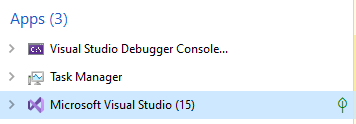
\includegraphics[scale=0.7]{before}
		\caption{Стан до створення процесів}
	\end{figure}
	
	\begin{figure}[H]
		\centering
		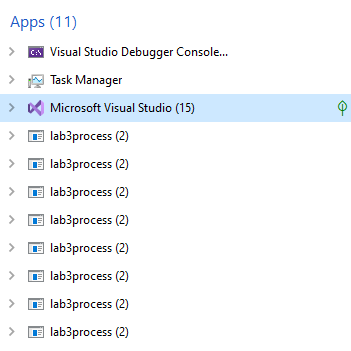
\includegraphics[scale=0.7]{after}
		\caption{Стан після створення процесів}
	\end{figure}
	
	\section*{Висновок}
	Під час виконання лабораторної роботи я ознайомився з багатопоточністю в ОС Windows. Навчився працювати з процесами, використовуючи WinAPI-функції. 
	
	Навчився створювати нові процеси, призупиняти, завершувати та продовжувати їх роботу.
	Навчився отримувати та встановлювати пріоритет процесу за допомогою Win-API функцій.
	Навчився отримувати час виконання процесу за допомогою Win-API функцій.
	
	 
\end{normalsize}
\end{document}
